%\documentclass[a4paper,twoside,11pt]{report}
\documentclass[a4paper,singleside,11pt]{report}

\usepackage[english]{babel}
\usepackage[utf8]{inputenc}
\usepackage[T1]{fontenc}
\usepackage{lmodern}

\usepackage[hidelinks]{hyperref}

\usepackage{tikz,
		    verbatim,
		    pgfplotstable,
		    float,
		    scrextend,
		    url,
		    rotating}
	    
\usetikzlibrary{positioning}

\usepackage[backend=bibtex,style=trad-plain, sorting=nty,firstinits=true]{biblatex}
\addbibresource{bibliography.bib}

\usepackage[formats]{listings}

\lstset{
	numbers = left,
	framexleftmargin=10mm,
	frame=none,
	backgroundcolor=\color[RGB]{245,245,245},
	showstringspaces=false,
	tabsize=2,
	breaklines=true
}

\begin{document}
	\title{A syllabification tool for very long poems in Italian\\
	\large Scala project for the Languages and Algorithms for Artificial Intelligence course}
	\author{Luca Salvatore Lorello\thanks{The author wishes to thank Mrs. Simona Scacchi, dutiful Italian teacher and friend, for her invaluable help.} (ID. 919584)}
	\date{Exam session: Summer 2020}
	\maketitle
	\tableofcontents
	
	\begin{abstract}
		This work aims to produce, given an Italian text, a syllabified version (with syllables separed by $\#$) of it, a dictionary of encountered syllables mapping each of them to their count, and order statistics on them (most frequent, least frequent and centiles).
		Peculiar aspects of the Italian language, in general, and of poetic style, in particular, are exploited to solve, up to a very satisfactory accuracy, the diphthong/hiatus ambiguity (which plays an important role in the syllabification process), and the algorithm is developed in order to be robust with respect to punctuation marks and capitalization.
		
		Albeit, clearly language dependent, the software architecture aims to be easily adaptable to one's needs, while remaining scalable. For this purpose, the syllable-splitting algorithm is implemented in a functional-programming style and different software architectures are explored.
		Furthermore some unit tests are implemented and the entire tool's scalability is benchmarked against long texts based on Dante's \emph{Commedia}.
	\end{abstract}
	
	\chapter{Problem analysis}

\section{Problem specification}
This project consists of a Scala tool capable of taking arbitrarily long Italian (with a particular focus on poetry) texts encoded in UTF-8 and returning a \emph{syllabified} version of them, in which all the syllable boundaries are marked with a $\#$ sign, while preserving other punctuation marks and being robust with respect to elisions~\cite{elision} (marked in Italian by the ' apostrophe) and metric dieresis~\cite{diaeresis} (marked in poetic Italian by an umlaut over vowels).
Since the algorithm processes \emph{written} Italian text, while syllabification is a \emph{phonological} phenomenon, the output's accuracy won't reach $100\%$, however synalepha~\cite{synalepha} phenomena will be detected as well.

Together with the syllabification of input texts, this project outputs some metrics measured on them:
\begin{itemize}
	\item Absolute count for each syllable (in a dictionary),
	\item Most frequent syllable,
	\item Median syllable,
	\item Least frequent syllable.
\end{itemize}

\section{Italian rules for syllabification}
A syllable is a group of phonemes which are emitted as a single sound. Any human language splits words into syllables in a process known as \emph{syllabification}, this process imposes constraints on the combinations of phonemes allowed in a given language.

As a universal principle, a syllable must contain at least a \emph{vocoid} and, optionally, antevocalic and/or postvocalic \emph{contoids}~\cite{demauro}. A single syllable is phonologically a variation of intensity in the sound emitted by the larynx, with \emph{peaks} corresponding to vocoids and \emph{troughs} corresponding to contoids, syllabification can therefore be analyzed phonetically by isolating each trough-to-trough segment of the voice intensity~\cite{maturileoni}.
Albeit simple and universal, this approach cannot be applied directly to written text, since the mapping between phonemes (sound units) and graphemes (text symbols) is not bijective, however in Italian vocoids always correspond to vowels (and therefore the first, and most important syllabification rule, can already be derived: a syllable must always contain at least a vowel) and the mapping presents very few exceptions.

For syllabification of a specific language, it's useful to use less general rules. Luckily, for the Italian language, these rules are well defined and only few cases of ambiguity arise when applied without phonetic informations (namely the position of the tonic accent inside words), moreover, heuristics exist for reducing these ambiguities further.

Before describing the syllabification rules for Italian, it's important to clarify some terms which will be used:
\begin{labeling}{Semiconsonant}
	\item [Digram] Sequence of two letters corresponding to a single sound, namely:
	\begin{itemize}
		\item gl + i, gn + vowel,
		\item sc + e/i,
		\item ch + e/i, gh + e/i,
		\item ci + a/o/u, gi + a/o/u (except when the i is accented, as in farmacìa).
	\end{itemize}
	\item [Trigram] Sequence of three letters corresponding to a single sound, namely:
	\begin{itemize}
		\item gli + a/o/u,
		\item sci + a/o/u.
	\end{itemize}
	\item [Semiconsonant] Vowel which is pronounced as if it was a consonant, can be only i/u in one of the following cases:
	\begin{itemize}
		\item i/u + accented vowel (eg. ièri, uòva, etc.),
		\item accented vowel + i/u,
		\item diphthongs,
		\item triphthongs.
	\end{itemize}
	\item [Diphthong] Sequence of two vowels pronounced with a single sound, namely:
	\begin{itemize}
		\item i + a/e/o/u,
		\item u + a/e/i/o,
		\item a/e/o/u + i,
		\item a/e + u.
	\end{itemize}
	\item [Triphthong] Sequence of three vowels pronounced with a single sound, namely:
	\begin{itemize}
		\item iài, ièi,
		\item uài, uòi, (eg. guài),
		\item iuò (eg. aiuòla).
	\end{itemize}
	\item [Hiatus] Sequence of two/three vowels pronounced separately, namely:
	\begin{itemize}
		\item a + e/o (eg. maestro),
		\item e + a/o,
		\item o + a/e,
		\item ì/ù + vowel(s) (eg. farmacìa, which is also an exception to the digram definition),
		\item ri/bi/tri + vowel (eg. biella),
		\item metric dieresis.
	\end{itemize}
	\item [Dieresis] In poetry, is a variation of pronunciation (for metric purposes) which splits letters which are usually pronounced together into multiple sounds, ie. a diphthong becomes a hiatus, as in ``così vid’ ïo la gloriosa rota'', where the syllable splitting is ``co-sì-vi-d’ï-o-la-glo-rio-sa-ro-ta'', instead of the prosaic split ``co-sì-vi-d’io-la-glo-rio-sa-ro-ta''.
	\item [Synalepha] In poetry, when a word ends with a vowel and the next one begins with another vowel, the two words are (often) merged into one and the boundary belongs to the same syllable (even if the joined vowels would normally form a hiatus, eg. ``Lì cominciò con forza e con menzogna'' is split as ``Lì-co-min-ciò-con-for-z\textbf{ae}-con-men-zo-gna'', even though a-e should be split, as in m\textbf{a-e}-stro).
\end{labeling}

From the above terminology, two sources of ambiguity \emph{arising when the accent is not marked} can be already be identified:
\begin{itemize}
	\item ci/gi + vowel can be either a digram (and so will be pronounced with the same sound as the vowel) or one of the possible hiatus cases (i + vowel, pronounced as two separate sounds),
	\item i/u + vowel can be either a diphthong or a hiatus.
\end{itemize}
Heuristics able to solve these ambiguities with an high precision exist, even when the accent is not explicitly marked~\cite{iato}, however since hiatuses are statistically rare in current Italian (pronunciation of languages tends towards simplification over time, and diphthongs are easier to pronounce than hiatuses), in case of ambiguity, the proposed algorithm will default to considering two consecutive vowels a diphthong.

Another ambiguity, which cannot be solved without semantic context (not even by humans), arises on deciding whether to apply a synalepha or not (this is at complete discretion of the poet and the same words, appearing in different verses can be tied by a synalepha in one and split in the other).
Since they are statistically frequent, the proposed algorithm will mark all the vocalic boundaries as possible synalepha.

The following rules are derived from~\cite{serianni,sensini}:
\begin{itemize}
	\item At the beginning of a word, a vowel or a diphthong form a syllable on their own (eg. \textbf{a}-mi-co, \textbf{au}-gu-ri, \textbf{e}-lo-qu-io),
	\item Diphthongs/triphthongs always belong to the same syllable (eg. a-\textbf{iuo}-la, u-ra-n\textbf{io}, ci-l\textbf{ie}-gia),
	\item Hiatuses (including dieresis, but excluding those appearing inside synalepha) are always split (eg. m\textbf{a-e}-stro, in-no-c\textbf{u-o}, in-vi-d\textbf{ï-o}-si, qu-\textbf{ï-e}-tar-mi),
	\item Digrams/trigrams are always together with the following vowel (eg. \textbf{ci}-lie-\textbf{gia}, \textbf{gno}-mo),
	\item A single consonant cannot be on it's own syllable (eg. \textbf{pa-lo}, a-\textbf{mi-co}),
	\item Double consonants (including cq) are always split (eg. a\textbf{c-q}ua, so\textbf{q-q}ua-dro, ri-du\textbf{r-r}e),
	\item Impure s (s + consonant) are always together with the following vowel (eg. \textbf{sce}l-le-ra-to, \textbf{sco}-\textbf{sta}r-si, \textbf{stra}p-pa-re),
	\item Other consecutive consonants are always split (eg. ac-cre-sci-me\textbf{n-t}o, a\textbf{n-t}ro-po-lo-gi-co), except when a mute consonant (b, c, d, g, p, t) is followed by a liquid one (l, r) (eg. pi-ro-\textbf{cla}-\textbf{sto}, ac-\textbf{cli}-ma-ta-to, an-\textbf{tro}-po-lo-gi-co, ac-\textbf{cre}-sci-men-to, s\textbf{tr}ap-pa-re), but not viceversa (cfr. a\textbf{r-t}o and an-\textbf{tr}o).
\end{itemize}

\section{Related work}
Nowadays any word processor or text preparation system ships with a syllabification engine, mainly used for correctly splitting a word near the page margin.

While syllabification principles are universal among human languages, the mapping between phonemes and graphemes is unique to each language and therefore different approaches need to be applied for each language.

The most used approach is based on lookup tables: each language has its own dictionary (which stores for each word its syllabification) and a newline is inserted at the closest splitting point. Although universal (and applicable to languages, like English, which don't have strict rules for mapping phonemes into graphemes), this approach tends not to scale well.
Rule-based approaches, like the one proposed in this project, are implemented in more sophisticated text preparation systems, like \LaTeX's \texttt{babel} package, and some computational linguistics pubblications~\cite{cioni,adsett}.
In text preparation systems the diphthong-hiatus ambiguity does not arise, thanks to the tendence of avoiding an end-of-line split between two vowels (no matter whether they form a diphthong or hiatus) in Italian, so a rule-based approach can be extremely compact and effective.
	\chapter{Software design}

\section{Word splitting procedure}
Syllabification is a sequential process which can be applied either to an entire text or to each word separately.
In order to exploit a distributed architecture, however, it's wise to apply the algorithm to single words (which can be distributed to different nodes, regardless of their actual position inside the text).

While prosaic text has a clear boundary between words (ie. a whitespace character), with the only exception of elisions (eg. ``l'amico'', which is considered a single word), poetic works tend to mimic the spoken tendency of joining consecutive words, by means of extensive use of \emph{synalepha} (which will alter the ``natural'' syllabification as well).

This requirement imposes to split the input into words when a whitespace (optionally with some punctuation marks, against which the procedure should be robust) is encountered, except in the following cases:
\begin{itemize}
	\item An apostrophe is encountered (either before, after or with no whitespace at all),
	\item The whitespace separates two vowels (except when a newline separates two verses).
\end{itemize}

In order to improve modularity, two splitting classes are implemented: the first one (actually a singleton object) splits the input into big \emph{chunks} (or \texttt{Pages}) of text (useful when the input is so big that even the word splitting procedure needs to be distributed); while the latter splits a single \texttt{Page} into words.

To improve code reuse, the shared splitting behavior is implemented in a \texttt{Splitter} trait which exposes a single \texttt{split(area: String): Queue[Int]} method taking an area of text and returning all the indexes in which a word split can be performed.
Internally it applies a tail-recursive split on whitespaces, checking whether the split found is acceptable or not according to the aforementioned criteria.

The \texttt{ChunkSplitter} object exposes two methods (\texttt{loadString(text: String, chunks: Int, lookahead: Int): Queue[Page]} and\\ \texttt{loadFile(file: String, chunks: Int, lookahead: Int):\\ Queue[Page]}) which load a text (from a string or a file respectively), applying a preliminary split into \texttt{Page} instances. An obvious race condition on the  input forces this initial split to be sequential, however, abstracting from loading overhead and assuming $\mathcal{O}(1)$ substring extraction by index, splits are performed (in a tail-recursive fashion) in $\mathcal{O}(\texttt{chunks} \cdot \texttt{lookahead})$ time, because the \texttt{ChunkSplitter} invokes the \texttt{split()} method only in substrings starting at $\texttt{i} \cdot \texttt{text.length()} / \texttt{chunks}$ and of length $\texttt{lookahead}$, for \texttt{i} in $0 .. \texttt{chunks} - 1$.

The \texttt{Page} case class models a single chunk of text. It's a string enriched with housekeeping informations required for later reconstruction of the original text, namely it's \texttt{id} and \texttt{start}/\texttt{end} indexes inside the original text, however in the current implementation these informations are not used, due to the word ordering being implicitly preserved during computations.

The \texttt{WordSplitter(val page: Page)} class' \texttt{getWords(): Queue[Word]} method splits words tail-recursively, producing an immutable queue of \texttt{Word}s.

\section{Syllable splitting rules}
Once words have been correctly split, their syllables can be computed independently on each of them, abstracting from their position inside the original text (as long as synalepha are considered a single word).
This property allows to encapsulate the syllable splitting inside the \texttt{Word} case class and to distribute its computation easily.

The \texttt{Word} case class exposes the methods \texttt{toSyllabifiedString(): String} and \texttt{toQueueOfSyllables(): Queue[Syllable]}, the former returns a string containing the word itself with syllables delimited by an $\#$ character, while the latter creates a \texttt{Syllable} instance for each syllable and stores them in a queue.

Each of them invokes private methods which split syllables in two phases:
\begin{enumerate}
	\item \texttt{performInitialSplits(str: String): String} (partially) splits syllables at easily identifiable boundaries:
	\begin{itemize}
		\item double consonants,
		\item multiple consonants,
		\item dieresis,
		\item hiatuses;
	\end{itemize}
	\item \texttt{performFinalSplits(str: String): String} splits syllables at harder to detect boundaries:
	\begin{itemize}
		\item contoid vocoid - contoid vocoid,
		\item vocoid - contoid vocoid,
		\item vocoid - vocoid.
	\end{itemize}
\end{enumerate}

As already discussed, ambiguities arise when two consecutive vowels meet, to solve this problem, heuristics need to be chosen:
\begin{itemize}
	\item \texttt{splitHiatus(str: String): String} splits only sure hiatuses (ie. those which can never be mistaken for diphthongs and those with a marked accent),
	\item \texttt{performFinalSplits(str: String): String} (in the vocoid - vocoid split) and the auxiliary method \texttt{clumpDiphthongs(str: String): String} consider two consecutive vowels diphthongs as often as possible (ie. when a sure triphthong cannot be detected), since hiatuses are already split when the method is invoked and the combination vowel + diphthong is statistically more common than a triphthong.
\end{itemize}

Since syllabification rules impose, not only splitting requirements (eg. between double consonants), but also clumping requirements, the special characters §, \{ and \} are internally used (and then removed) to mark positions in which a split is forbidden, therefore these characters (along with $\#$) should not appear in the input text.


\section{Frequency analysis}
In order to unify every possible variant of a \texttt{Syllable} (eg. uppercase, lowercase, with apostrophes, with diacritics, inside synalepha, etc.), a\\ \texttt{CharacterSequence} trait (which is mixed-in \texttt{Page} and \texttt{Word} classes as well) is injected in the \texttt{Syllable} case class.

\texttt{CharacterSequence}'s \texttt{toPrettyString(): String} method converts the \texttt{str} attribute of the injected class to a lowercase version, without spaces, punctuation marks and diacritics (accents and dieresis) on vowels.
The \texttt{toString(): String} method overrides the default behavior returning the \texttt{str} attribute for convenience.

\subsection{Syllable count}
The most natural way of counting elements of a collection of elements of type \texttt{K} is to use any collection implementing the \texttt{Map[K, Int]} trait, indexed with the distinct elements of the collection.
This approach works reasonably fast (since it can be performed in $\mathcal{O}(n)$) as long as indexing can be performed in $\mathcal{O}(1)$ (which is the case for \texttt{HashMap}, the default implementation of \texttt{Map}).

\texttt{Map}s typically impose constraints on the key type, in the case of \texttt{HashMap} it must be hashable, ie. each element should be uniquely identified (and its identifier must never change during the collection's lifetime). Since \texttt{String} is an immutable type, a prettified \texttt{CharacterSequence} satisfies both the language specifications and the ``semantic'' requirement of aggregating different versions of the same syllable (eg. ``l'a'' and ``la'' are prettified in the same way and therefore counted together).

\subsection{Order statistics}
While selection algorithms (eg. Quickselect, Heapselect, etc.) have an average complexity of $\mathcal{O}(n)$, the need of extracting more than one selection statistic neglects their advantage over the ``naive'' sort ($\mathcal{O}(n log(n))$) followed by indexing ($\mathcal{O}(1)$), the latter strategy is therefore preferred.


\section{Integration and distributed architecture}
Although the syllabified output is intrinsically sequential and the map of syllable occurrences is a shared resource in which multiple agents need to synchronize, the implementation will benefit from parallel or distributed execution. To prove this claim, the same algorithm is implemented in multiple architectures and their performance will be profiled to determine which scales better with respect to input size.

In general the workflow is to split the input into \texttt{Page}s, each page into \texttt{Word}s and each word into \texttt{Syllable}s. In order to preserve the ordering, the most natural choice for collections is the \texttt{Queue}, using its \emph{immutable} variant allows to distribute its content in a straight forward manner, since it can be handled in a purely functional fashion.

\begin{lstlisting}[mathescape=true,language=scala, caption={Syllable extraction pseudocode}]
val pages: Queue[Page] = ChunkSplitter.loadFile(in, chunks, lookahead)
val wordSplitters: Queue[WordSplitter] = pages.map(p => new WordSplitter(p))
val words: Queue[Word] = wordSplitters.flatMap(ws => w.getWords())
val syllables: Queue[Syllable] = words.flatMap(w => w.toQueueOfSyllables())
\end{lstlisting}

Once the queue of syllables is obtained, two substantially different operations need to be performed:
\begin{itemize}
	\item Output the queue as a string,
	\item Count the occurrences of each syllable.
\end{itemize}

While the first operation requires to preserve positional information on each syllable (implicitly encoded by a syllable's position inside the queue), the latter can be efficiently computed only after aggregation, it's therefore more reasonable to compute them in the aforementioned order, instead of recomputing positions which will be inevitably lost during aggregation.

The first output can be simply computed exploiting the method\\ \texttt{Seq.mkstring(str: String)} on the queue of syllables, or using directly the method \texttt{Word.toSyllabifiedString()} mapping each word into a string and then joining them.

The second output involves unification of different variants of the same syllable and the creation of the occurrence map.
The last step can be performed by creating an intermediate queue of \texttt{Tuple2[String, Int]}, which associates each syllable to a single occurrence, and then aggregating all the tuples with the same key by summing their values.

\begin{lstlisting}[mathescape=true,language=scala, caption={Syllable counting pseudocode}]
val prettySyllables: Queue[String] = syllables.map(s => s.toPrettyString)
val tuples: Queue[(String, Int)] = prettySyllables.map (ps => (ps, 1))
val count: Map[String, Int] = tuples.reduceByKey((a, b) => a + b)
\end{lstlisting}

While this implementation looks straightforward, the method \texttt{reduceByKey} is not a native Scala method (it's implemented by Spark's framework) and a less abstract implementation needs to be performed: a queue of queues is computed by grouping each tuple by their key (the first element) and then each subqueue is mapped into a new tuple \texttt{(key, sum of values)}.

\begin{lstlisting}[mathescape=true,language=scala, caption={reduceByKey pseudocode}]
val queueOfQueues = tuples.groupBy(t => t._1)
val count: Map[String, Int] = queueOfQueues.mapValues(el => el.map(t => t._2).sum)
\end{lstlisting}

In case of multiple pages, a partial occurrence count for each of them can be obtained. In order to merge them, a reduction is performed by summing, for each key in the concatenated map (which overwrites duplicate keys with the value from the second map), the corresponding value with either the value of the first map (if the key was duplicated) or zero.

\begin{lstlisting}[mathescape=true,language=scala, caption={Map merging pseudocode}]
val count: Map[String, Int] = queueOfCounts.reduce(
	(m1, m2) => m1 ++ m2.map {
		case (k, v) => k -> (v + m1.getOrElse(k, 0))
	}
)
\end{lstlisting}

The occurrence count map is finally sorted and centiles are extracted as output.

\subsection{Sequential architecture}
\begin{figure}[H]
	\center
	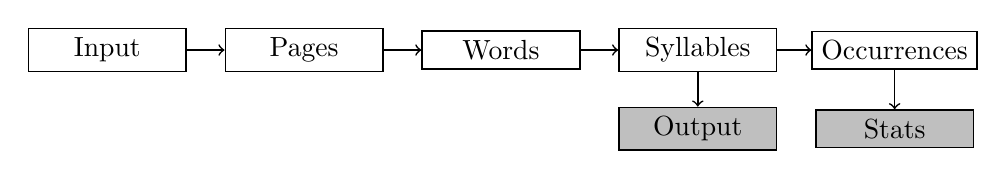
\begin{tikzpicture}[->, auto, node distance=1cm and 2.5cm, on grid, semithick, state/.style={draw, black, minimum width=2cm}]
	\node[state] (A) []{Input};
	\node[state] (B) [right= of A]{Pages};
	\node[state] (C) [right= of B]{Words};
	\node[state] (D) [right= of C]{Syllables};
	\node[state, fill=lightgray] (E) [below=of D]{Output};
	\node[state] (F) [right=of D]{Occurrences};
	\node[state, fill=lightgray] (G) [below= of F]{Stats};
	
	\path (A) edge[] node[]{} (B);
	\path (B) edge[] node[]{} (C);
	\path (C) edge[] node[]{} (D);
	\path (D) edge[] node[]{} (E);
	\path (D) edge[] node[]{} (F);
	\path (F) edge[] node[]{} (G);
	
	\end{tikzpicture}
	\caption{Sequential dataflow}
	\label{fig:seq}
\end{figure}

In this straightforward architecture, a single computational unit is used to proceed from input to outputs.
Even though the input can be split into multiple pages (and therefore partial occurrence maps can be computed for each of them), processing is performed in order.

\subsection{Parallel architecture}
\begin{figure}[H]
	\center
	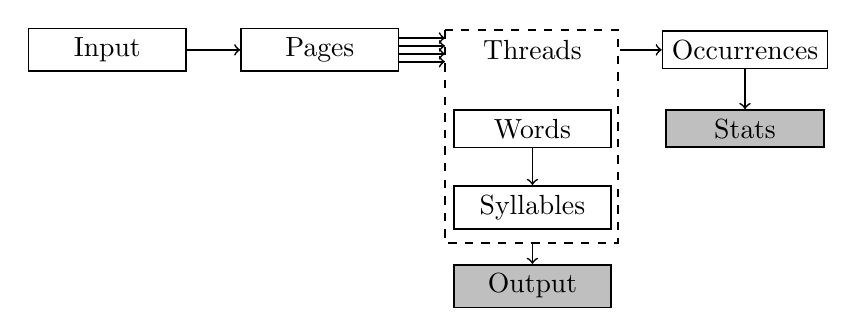
\begin{tikzpicture}[->, auto, node distance=1cm and 2.7cm, on grid, semithick, state/.style={draw, black, minimum width=2cm}, thread/.style={black, minimum width=2.2cm}]
	\node[state] (A) []{Input};
	\node[state] (B) [right= of A]{Pages};
	\node[thread] (T) [right= of B] {Threads};
	\node[state] (C) [below= of T]{Words};
	\node[state] (D) [below= of C]{Syllables};
	\node[state, fill=lightgray] (E) [below=of D]{Output};
	\node[state] (F) [right=of T]{Occurrences};
	\node[state, fill=lightgray] (G) [below=of F]{Stats};

	\draw [dashed](T.north west) rectangle +(2.2cm, -2.7cm);
		
	\path (A) edge[] node[]{} (B);
	\path (C) edge[] node[]{} (D);
	\path (T) edge[] node[]{} (F);
	\path (F) edge[] node[]{} (G);
	
	\draw ([yshift=0.15cm]B.east) -> ([yshift=0.15cm]T.west);
	\draw ([yshift=0.05cm]B.east) -> ([yshift=0.05cm]T.west);
	\draw ([yshift=-0.05cm]B.east) -> ([yshift=-0.05cm]T.west);
	\draw ([yshift=-0.15cm]B.east) -> ([yshift=-0.15cm]T.west);
	
	\draw ([yshift=-2.2cm]T.south) -> ([]E.north);
	
	\end{tikzpicture}
	\caption{Parallel dataflow}
	\label{fig:par}
\end{figure}

Since syllabification is an instance of an \emph{embarassingly parallel}~\cite{embarassing} task, a parallel architecture can be devised, with no need for synchronization mechanisms, other than a \emph{barrier} at the end of each computation.

In this architecture, a worker \emph{thread} is started for each page. When syllabification is completed for the associated page, each thread stores internally the final results (the syllabified string and a partial occurrence count).
When every thread has finished, the partial results are merged together sequentially (a simple append in the case of the syllabified output, a reduction for the partial occurrence maps).

\subsection{First distributed architecture}
\begin{figure}[H]
	\center
	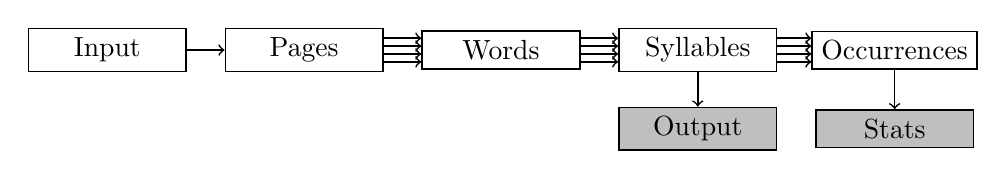
\begin{tikzpicture}[->, auto, node distance=1cm and 2.5cm, on grid, semithick, state/.style={draw, black, minimum width=2cm}]
	\node[state] (A) []{Input};
	\node[state] (B) [right= of A]{Pages};
	\node[state] (C) [right= of B]{Words};
	\node[state] (D) [right= of C]{Syllables};
	\node[state, fill=lightgray] (E) [below=of D]{Output};
	\node[state] (F) [right=of D]{Occurrences};
	\node[state, fill=lightgray] (G) [below= of F]{Stats};
	
	\path (A) edge[] node[]{} (B);
	\path (F) edge[] node[]{} (G);
	
	\draw ([yshift=0.15cm]B.east) -> ([yshift=0.15cm]C.west);
	\draw ([yshift=0.05cm]B.east) -> ([yshift=0.05cm]C.west);
	\draw ([yshift=-0.05cm]B.east) -> ([yshift=-0.05cm]C.west);
	\draw ([yshift=-0.15cm]B.east) -> ([yshift=-0.15cm]C.west);
	
	\draw ([yshift=0.15cm]C.east) -> ([yshift=0.15cm]D.west);
	\draw ([yshift=0.05cm]C.east) -> ([yshift=0.05cm]D.west);
	\draw ([yshift=-0.05cm]C.east) -> ([yshift=-0.05cm]D.west);
	\draw ([yshift=-0.15cm]C.east) -> ([yshift=-0.15cm]D.west);
	
	\draw ([yshift=0.15cm]D.east) -> ([yshift=0.15cm]F.west);
	\draw ([yshift=0.05cm]D.east) -> ([yshift=0.05cm]F.west);
	\draw ([yshift=-0.05cm]D.east) -> ([yshift=-0.05cm]F.west);
	\draw ([yshift=-0.15cm]D.east) -> ([yshift=-0.15cm]F.west);
	
	\draw ([]D.south) -> ([]E.north);
	
	\end{tikzpicture}
	\caption{Distributed dataflow with maximum parallelism}
	\label{fig:spark1}
\end{figure}

Since every collection involved in the program is immutable, they can be parallelized into Spark's resilient distributed datasets and the output can be computed in a distributed fashion.

Data distribution can be implemented in two possible ways, by maximizing parallelism or by minimizing inter-node communication.
The former approach is discussed in this section, while the latter in the following.

Since the disk is a shared resource, pages still need to be split sequentially, however as soon as a \texttt{WordSplitter} can be created for each of them, the collection can be distributed.

RDD transformations create two new RDDs (of words first and then of syllables), then the syllabified output is collected and the same RDD of syllables is further transformed into an RDD of occurrences (which is sorted by the distributed framework prior to collection).

While this approach tends to maximize the amount of data which is processed simultaneously, the first two transformations \textbf{increase} the number of elements (contrary to the usual approach of trying to reduce an RDD size at each step, to minimize communication, which is the bottleneck of this architecture), making this architecture potentially slow in some circumstances.

\subsection{Second distributed architecture}
\begin{figure}[H]
	\center
	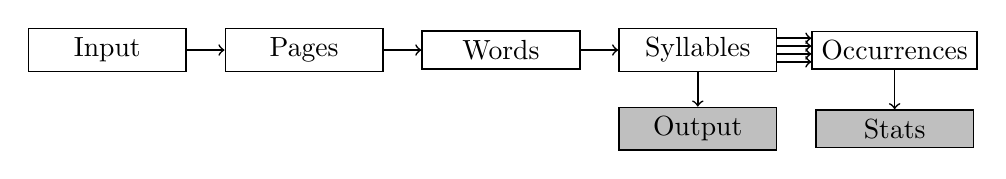
\begin{tikzpicture}[->, auto, node distance=1cm and 2.5cm, on grid, semithick, state/.style={draw, black, minimum width=2cm}]
	\node[state] (A) []{Input};
	\node[state] (B) [right= of A]{Pages};
	\node[state] (C) [right= of B]{Words};
	\node[state] (D) [right= of C]{Syllables};
	\node[state, fill=lightgray] (E) [below=of D]{Output};
	\node[state] (F) [right=of D]{Occurrences};
	\node[state, fill=lightgray] (G) [below= of F]{Stats};
	
	\path (A) edge[] node[]{} (B);
	\path (B) edge[] node[]{} (C);
	\path (C) edge[] node[]{} (D);
	\path (F) edge[] node[]{} (G);
	
	\draw ([yshift=0.15cm]D.east) -> ([yshift=0.15cm]F.west);
	\draw ([yshift=0.05cm]D.east) -> ([yshift=0.05cm]F.west);
	\draw ([yshift=-0.05cm]D.east) -> ([yshift=-0.05cm]F.west);
	\draw ([yshift=-0.15cm]D.east) -> ([yshift=-0.15cm]F.west);
	
	\draw ([]D.south) -> ([]E.north);
	
	\end{tikzpicture}
	\caption{Distributed dataflow with minimum parallelism}
	\label{fig:spark2}
\end{figure}

By postponing parallelization as much as possible, it's possible to minimize communication, at the expenses of a lower degree of parallelism.

This architecture produces a queue of syllables sequentially and then parallelizes it into an RDD in order to perform only the last transformation into an RDD of occurrences.

This seemingly naive implementation is in fact better than the previous one, in case the trade off between network communication and sequential syllabification is heavily shifted in favor of the latter.
	\chapter{Tests}

\section{Unit tests}
The \texttt{Scalatest} framework was used to perform some unit tests which drove the development of word and syllable splitting algorithms.

Namely, four \texttt{FunSuite}s were implemented in order to test:
\begin{itemize}
	\item the \texttt{CharacterSequence} trait behavior,
	\item the \texttt{Splitter} trait behavior,
	\item the syllabification of single words,
	\item the syllabification of entire verses.
\end{itemize}

Although complete coverage was not reached, test cases covered both common and exotic inputs, and all tests except two (caused by a failure of the chosen heuristics for those inputs) passed.

\section{Profiling}

In order to time the execution of the four proposed architectures, a \texttt{Profiler} trait was implemented and, in order to achieve higher granularity, their implementation was split into functions profiled separately.

The \texttt{Profiler} trait exposes two higher order methods: \texttt{profile[T](f: => T): (T, Long)} takes a function and times its execution (returning its return value and the time taken in nanoseconds), exploiting call-by-name parameter passing for a correct profiling, \texttt{smoothProfile[T](f: => T, times: Int): (T, Long)} profiles the function more than once and returns the average time (together with the last return value) in order to filter out noise caused by other processes running on the machine.

While optimization could not be turned off (many methods are tail recursive, therefore a compiler optimization is needed for large inputs), the tests have been performed on a fresh virtual machine (with no processes running other than the system daemons) mapped to 4 CPU cores (with $100 \%$ execution cap on the physical hardware) and $8 Gb$ of RAM, and averaged over multiple runs whenever applicable (neither the distributed architectures nor the tests on large inputs are averaged, the formers to avoid underestimating execution time due to caching, the latters due to lack of time).

An initial implementation used \texttt{List}s instead of \texttt{Queue}s, in order to make the code ``more functional'', however their poor performance (every append operation worked, especially using only the \texttt{::} operator, in $\mathcal{O}(n)$, while queues can \texttt{enqueue} in $\mathcal{O}(1)$) ultimately lead to ruling them out.
The following benchmarks are performed on both implementations, showing the dominance of performance of queues over lists also in practice, in terms of execution time.

The benchmarks were performed on the following files:
\begin{itemize}
	\item \texttt{La Divina Commedia.txt} composed of 561097 UTF-8 characters,
	\item \texttt{La Divina Commedia large.txt} composed of 2805485 UTF-8 characters (original dataset copy-pasted 5 times),
	\item \texttt{La Divina Commedia huge.txt} composed of 5610970 UTF-8 characters (original dataset copy-pasted 10 times),
	\item in memory strings generated by appending programmatically \texttt{La Divina Commedia.txt} to itself between 1 and 20 times.
\end{itemize}

\subsection{General assessment}

A preliminary assessment was performed in order to compare the performance of list-based and queue-based implementations.

The following is the output for lists (related only to the original dataset):
\begin{verbatim}
Profiling the sequential execution on file "La Divina Commedia.txt",
    split into 4 chunks (profiling averaged over 5 runs)...
Total (averaged) running time: 47921.384041 ms, of which:
  43.373189 ms for reading the file and splitting into chunks,
  47829.655373 ms for splitting each word into syllables and building
    a dictionary of occurrences for each chunk,
  35.288367 ms for merging the dictionaries into one,
  13.067112 ms for sorting and extracting the centiles.

Profiling the parallel execution on file "La Divina Commedia.txt",
    split into 4 chunks (profiling averaged over 5 runs).
    Each chunk is processed by a different thread...
Total (averaged) running time: 22331.325159 ms, of which:
  4.747231 ms for reading the file and splitting into chunks (sequential),
  22294.380319 ms for splitting each word into syllables and building a
    dictionary of occurrences for each chunk (parallel),
  23.938964 ms for merging the dictionaries into one (sequential),
  8.258645 ms for sorting and extracting the centiles (sequential).

Profiling the distributed execution on file "La Divina Commedia.txt",
    split into 4 chunks (profiling CANNOT be averaged).
    Each chunk is processed by a different node...
Total (averaged) running time: 28251.505847 ms, of which:
  2071.806305 ms for initializing Spark,
  455.901307 ms for reading the file and splitting into chunks (sequential),
  12477.873347 ms for splitting each word into syllables and building a
    dictionary of occurrences for each chunk (distributed),
  13245.924888 ms for sorting and extracting the centiles and shutting down
    Spark (sequential).

Profiling the distributed execution on file "La Divina Commedia.txt"
    with no prior splitting (profiling CANNOT be averaged).
    The number of nodes is chosen by Spark...
Total (averaged) running time: 87137.502624 ms, of which:
  94.868064 ms for initializing Spark,
  85781.084591 ms for reading the file, splitting into syllables and
    distributing the dataset (sequential),
  68.578017 ms for building a dictionary of occurrences (distributed),
  1192.971952 ms for sorting, extracting the centiles and shutting down
    Spark (sequential).
\end{verbatim}

As it can be noted, for every implementation, the slowest operation is the syllable splitting procedure, however a clear advantage is achieved when exploiting parallelism.
The number of pages the input is split into also relates to the performance of the merge procedure (slower when merging fewer occurrence maps of large size, instead of many smaller maps), this hints a non-linear, probably polynomial, complexity (since $m\cdot\mathcal{T}(n/m) \ll \mathcal{T}(n)$).


The following is the output for queues (on the same input file):
\begin{verbatim}
Profiling the sequential execution on file "La Divina Commedia.txt",
    split into 4 chunks (profiling averaged over 5 runs)...
Total (averaged) running time: 31229.42195 ms, of which:
  59.813815 ms for reading the file and splitting into chunks,
  31101.113841 ms for splitting each word into syllables and building a
    dictionary of occurrences for each chunk,
  54.814361 ms for merging the dictionaries into one,
  13.679933 ms for sorting and extracting the centiles.

Profiling the parallel execution on file "La Divina Commedia.txt",
    split into 4 chunks (profiling averaged over 5 runs).
    Each chunk is processed by a different thread...
Total (averaged) running time: 13635.397876 ms, of which:
  4.850249 ms for reading the file and splitting into chunks (sequential),
  13585.609283 ms for splitting each word into syllables and building a
    dictionary of occurrences for each chunk (parallel),
  35.490544 ms for merging the dictionaries into one (sequential),
  9.4478 ms for sorting and extracting the centiles (sequential).

Profiling the distributed execution on file "La Divina Commedia.txt",
    split into 4 chunks (profiling CANNOT be averaged).
    Each chunk is processed by a different node...
Total (averaged) running time: 19099.583035 ms, of which:
  2420.161538 ms for initializing Spark,
  240.389256 ms for reading the file and splitting into chunks (sequential),
  8209.232922 ms for splitting each word into syllables and building a
    dictionary of occurrences for each chunk (distributed),
  8229.799319 ms for sorting and extracting the centiles and shutting down
    Spark (sequential).

Profiling the distributed execution on file "La Divina Commedia.txt"
    with no prior splitting (profiling CANNOT be averaged).
    The number of nodes is chosen by Spark...
Total (averaged) running time: 76563.562394 ms, of which:
  171.860143 ms for initializing Spark,
  75096.973943 ms for reading the file, splitting into syllables
    and distributing the dataset (sequential),
  53.080434 ms for building a dictionary of occurrences (distributed),
  1241.647874 ms for sorting, extracting the centiles and shutting down
    Spark (sequential).
\end{verbatim}

The execution times are sensibly lower, demonstrating that the $\mathcal{O}(n)$ list append effectively acted as a bottleneck on most operations (including RDD transformations).

Further tests on the two implementations were run using the three datasets loaded from disk, in order to show the effect of varying input size.

\begin{figure}[H]
	\center
	\resizebox{\textwidth}{!}{
		\begin{tikzpicture}
		\begin{semilogyaxis}[axis lines=middle, xmin=0, xmax=10, ymin=0, ymax=3500,samples=1000, xtick={1,5,10}, xlabel={Dataset size}, ylabel={Running time (s)}, legend style={font=\tiny},
		x label style={at={(axis description cs:0.5,-0.1)},anchor=north},
		y label style={at={(axis description cs:-0.1,.5)},rotate=90,anchor=south},
		tick label style={font=\tiny},
		label style={font=\tiny},
		legend pos=outer north east,
		legend entries={Sequential, Parallel (4 thds), Parallel (20 thds), Spark 1 (4 nodes), Spark 1 (20 nodes), Spark 2}]
		\addplot[
		ultra thin,
		scatter,
		point meta=explicit symbolic,
		forget plot,
		scatter/classes={
			seql={mark=+, draw=black,mark size=2}
		}
		]
		file{data/seql.txt};
		\addplot[
		ultra thin,
		scatter,
		point meta=explicit symbolic,
		forget plot,
		scatter/classes={
			par4l={mark=o, draw=black,mark size=2}
		}
		]
		file{data/par4l.txt};
		\addplot[
		ultra thin,
		scatter,
		point meta=explicit symbolic,
		forget plot,
		scatter/classes={
			par20l={mark=diamond, draw=black,mark size=2}
		}
		]
		file{data/par20l.txt};
		\addplot[
		ultra thin,
		scatter,
		point meta=explicit symbolic,
		forget plot,
		scatter/classes={
			spark14l={mark=square, draw=black,mark size=2}
		}
		]
		file{data/spark14l.txt};
		\addplot[
		ultra thin,
		scatter,
		point meta=explicit symbolic,
		forget plot,
		scatter/classes={
			spark120l={mark=asterisk, draw=black,mark size=2}
		}
		]
		file{data/spark120l.txt};
		\addplot[
		ultra thin,
		scatter,
		point meta=explicit symbolic,
		forget plot,
		scatter/classes={
			spark2l={mark=triangle, draw=black,mark size=2}
		}
		]
		file{data/spark2l.txt};
		\addlegendimage{mark=+}
		\addlegendimage{mark=o}
		\addlegendimage{mark=diamond}
		\addlegendimage{mark=square}
		\addlegendimage{mark=asterisk}
		\addlegendimage{mark=triangle}
		\end{semilogyaxis}
		\end{tikzpicture}
	}
	\caption{Scalability of execution times on list-based implementations}
	\label{fig:listsemilog}
\end{figure}

\begin{figure}[H]
	\center
	\resizebox{\textwidth}{!}{
		\begin{tikzpicture}
		\begin{semilogyaxis}[axis lines=middle, xmin=0, xmax=10, ymin=0, ymax=3500,samples=1000, xtick={1,5,10}, xlabel={Dataset size}, ylabel={Running time (s)}, legend style={font=\tiny},
		x label style={at={(axis description cs:0.5,-0.1)},anchor=north},
		y label style={at={(axis description cs:-0.1,.5)},rotate=90,anchor=south},
		tick label style={font=\tiny},
		label style={font=\tiny},
		legend pos=outer north east,
		legend entries={Sequential, Parallel (4 thds), Parallel (20 thds), Spark 1 (4 nodes), Spark 1 (20 nodes), Spark 2}]
		\addplot[
		ultra thin,
		scatter,
		point meta=explicit symbolic,
		forget plot,
		scatter/classes={
			seqq={mark=+, draw=black,mark size=2}
		}
		]
		file{data/seqq.txt};
		\addplot[
		ultra thin,
		scatter,
		point meta=explicit symbolic,
		forget plot,
		scatter/classes={
			par4q={mark=o, draw=black,mark size=2}
		}
		]
		file{data/par4q.txt};
		\addplot[
		ultra thin,
		scatter,
		point meta=explicit symbolic,
		forget plot,
		scatter/classes={
			par20q={mark=diamond, draw=black,mark size=2}
		}
		]
		file{data/par20q.txt};
		\addplot[
		ultra thin,
		scatter,
		point meta=explicit symbolic,
		forget plot,
		scatter/classes={
			spark14q={mark=square, draw=black,mark size=2}
		}
		]
		file{data/spark14q.txt};
		\addplot[
		ultra thin,
		scatter,
		point meta=explicit symbolic,
		forget plot,
		scatter/classes={
			spark120q={mark=asterisk, draw=black,mark size=2}
		}
		]
		file{data/spark120q.txt};
		\addplot[
		ultra thin,
		scatter,
		point meta=explicit symbolic,
		forget plot,
		scatter/classes={
			spark2q={mark=triangle, draw=black,mark size=2}
		}
		]
		file{data/spark2q.txt};
		\addlegendimage{mark=+}
		\addlegendimage{mark=o}
		\addlegendimage{mark=diamond}
		\addlegendimage{mark=square}
		\addlegendimage{mark=asterisk}
		\addlegendimage{mark=triangle}
		\end{semilogyaxis}
		\end{tikzpicture}
	}
	\caption{Scalability of execution times on queue-based implementations}
	\label{fig:queuesemilog}
\end{figure}

For both implementations, it can be noted how the second Spark implementation (minimum inter-node communication) scales the worst, followed by low-parallelism implementations (parallel architecture and the first Spark implementation with few nodes).
The best scalability is achieved by the sequential implementation and high-parallelism implementations, hinting the fact that for increasing datasets, the occurrence map merging operation becomes more and more relevant for the overall performance (the sequential implementation doesn't need to merge anything, while high-parallelism implementations need to merge only small-sized maps).

\subsection{Execution time with respect to degree of parallelism}
In order to further investigate the dependency of execution times with respect to the degree of parallelism, the parallel architecture was tested using a fixed input (the original dataset), varying the number of threads.

\begin{figure}[H]
	\center
	\resizebox{\textwidth}{!}{
		\begin{tikzpicture}
		\begin{axis}[axis lines=middle, xmin=0, xmax=100, ymin=0, ymax=70,samples=1000, xtick={0,10,...,100}, xlabel={Number of threads}, ylabel={Running time (s)}, legend style={font=\tiny},
		x label style={at={(axis description cs:0.5,-0.1)},anchor=north},
		y label style={at={(axis description cs:-0.1,.5)},rotate=90,anchor=south},
		tick label style={font=\tiny},
		label style={font=\tiny},
		legend pos=outer north east,
		legend entries={Using lists, Using queues}]
		\addplot[
		ultra thin,
		scatter,
		point meta=explicit symbolic,
		forget plot,
		scatter/classes={
			lists={mark=+,draw=black,mark size=2}
		}
		]
		file{data/threads_lists.txt};
		\addplot[
		ultra thin,
		scatter,
		point meta=explicit symbolic,
		forget plot,
		scatter/classes={
			queues={mark=o, draw=black,mark size=2}
		}
		]
		file{data/threads_queues.txt};
		\addlegendimage{mark=+}
		\addlegendimage{mark=o}
		\end{axis}
		\end{tikzpicture}
	}
	\caption{Efficiency with respect to the number of threads}
	\label{fig:threads}
\end{figure}

It is important to notice that JVM's mapping is many-to-many, so the number of threads effectively running simultaneously will depend on the system's load, however it will never exceed the number of CPUs available on the machine (4 in this case).
As such, the expected performance (on the parallel component only) should converge pretty soon (and after a given threshold context-switching overhead should cause a performance degradation).

Although this convergence can be clearly seen on the plot, it doesn't happen as soon as expected, due to the combination with the performance of the sequential part of the implementation (namely the occurrence maps merging, which, as stated before, performs better when merging many smaller maps instead of few larger ones).

Finally, as already demonstrated, the list-based implementation is in all cases outperformed by the queue-based one.

\subsection{Comparing the most promising architectures}
A final test was performed comparing the most promising architectures (sequential, parallel implementation with 20 threads and Spark implementation with maximal parallelism using 20 nodes) on the queue-based implementation to better assess the scalability.

The input was given a a string obtained by repeatedly concatenating in RAM the original dataset a given number of times, due to this lack of I/O operations and the fact that the complete architectures were profiled in a single function for each of them, compiler optimization achieved different results than the other tests (element-wise figures in this test are smaller than the ones obtained in other tests), however the general trend is preserved.

The sequential implementation clearly diverges from the other two, the larger the input becomes, while the parallel implementations tend to perform similarly (this is justified by the fact that on a single machine Spark will still be subjected to the same hardware limitations as the multithreaded implementation, and due to the fact that its core is not completely shut down between each experiment, leading to warm-restarts).

For clarity, both a linear and a semilog plot of the same results are shown, from both a polynomial trend clearly emerges.

\begin{sidewaysfigure}
	\center
	\resizebox{\textwidth}{!}{
		\begin{tikzpicture}
		\begin{axis}[axis lines=middle, xmin=0, xmax=20, ymin=0, ymax=3500,samples=1000, xtick={1,5,10,15,20}, xlabel={Dataset size}, ylabel={Running time (s)}, legend style={font=\tiny},
		x label style={at={(axis description cs:0.5,-0.1)},anchor=north},
		y label style={at={(axis description cs:-0.1,.5)},rotate=90,anchor=south},
		tick label style={font=\tiny},
		label style={font=\tiny}]
		\addplot[
		ultra thin,
		scatter,
		point meta=explicit symbolic,
		forget plot,
		scatter/classes={
			seqq={mark=+, draw=black,mark size=2}
		}
		]
		file{data/seqq_2.txt};
		\addplot[
		ultra thin,
		scatter,
		point meta=explicit symbolic,
		forget plot,
		scatter/classes={
			par20q={mark=diamond, draw=black,mark size=2}
		}
		]
		file{data/par20q_2.txt};
		\addplot[
		ultra thin,
		scatter,
		point meta=explicit symbolic,
		forget plot,
		scatter/classes={
			spark120q={mark=asterisk, draw=black,mark size=2}
		}
		]
		file{data/spark120q_2.txt};
		\end{axis}
		\end{tikzpicture}
		\begin{tikzpicture}
		\begin{semilogyaxis}[axis lines=middle, xmin=0, xmax=20, ymin=0, ymax=3500,samples=1000, xtick={1,5,10,15,20}, xlabel={Dataset size}, ylabel={Running time (s)}, legend style={font=\tiny},
		x label style={at={(axis description cs:0.5,-0.1)},anchor=north},
		y label style={at={(axis description cs:-0.1,.5)},rotate=90,anchor=south},
		tick label style={font=\tiny},
		label style={font=\tiny},
		legend pos=outer north east,
		legend entries={Sequential, Parallel (20 thds), Spark 1 (20 nodes)}]
		\addplot[
		ultra thin,
		scatter,
		point meta=explicit symbolic,
		forget plot,
		scatter/classes={
			seqq={mark=+, draw=black,mark size=2}
		}
		]
		file{data/seqq_2.txt};
		\addplot[
		ultra thin,
		scatter,
		point meta=explicit symbolic,
		forget plot,
		scatter/classes={
			par20q={mark=diamond, draw=black,mark size=2}
		}
		]
		file{data/par20q_2.txt};
		\addplot[
		ultra thin,
		scatter,
		point meta=explicit symbolic,
		forget plot,
		scatter/classes={
			spark120q={mark=asterisk, draw=black,mark size=2}
		}
		]
		file{data/spark120q_2.txt};
		\addlegendimage{mark=+}
		\addlegendimage{mark=diamond}
		\addlegendimage{mark=asterisk}
		\end{semilogyaxis}
		\end{tikzpicture}
	}
	\caption{Running time of the queue-based implementation}
	\label{fig:topolino}
\end{sidewaysfigure}

	
	\appendix
	
	\lstlistoflistings
	
	\printbibliography % biblatex
\end{document}